%++++++++++++++++++++++++++++++++++++++++
\documentclass[article, 12pt]{article}
\usepackage{float}
\usepackage{setspace}
\usepackage{tabu} % extra features for tabular environment
\usepackage{amsmath}  % improve math presentation
\usepackage{graphicx} % takes care of graphic including machinery
\usepackage[margin=1in]{geometry} % decreases margins
\usepackage{cite} % takes care of citations
\usepackage[final]{hyperref} % adds hyper links inside the generated pdf file
\usepackage{tikz}
\usepackage{caption} 
\usepackage{fancyhdr}
\usepackage{amssymb} % symbols like /therefore
\usepackage{amsthm} % proofs
\usepackage{enumerate} % lettered lists
\usepackage{mathtools} % macros
\usetikzlibrary{scopes}
% \usepackage{xcolor} \pagecolor[rgb]{0.12549019607,0.1294117647,0.13725490196} \color[rgb]{0.82352941176,0.76862745098,0.62745098039} % dark theme
\theoremstyle{definition}
\newtheorem{example}{Example}[subsubsection]
\newtheorem*{remark}{Remark}
\newtheorem{theorem}{Theorem}[subsubsection]
\newtheorem{definition}{Definition}[subsubsection]
\newtheorem{corollary}{Corollary}[subsubsection]
\hypersetup{
	colorlinks=false,      % false: boxed links; true: colored links
	linkcolor=blue,        % color of internal links
	citecolor=blue,        % color of links to bibliography
	filecolor=magenta,     % color of file links
	urlcolor=blue         
}
\usepackage{physics}
\usepackage{siunitx}
\usepackage{tikz,pgfplots}
\usepackage[outline]{contour} % glow around text
\usetikzlibrary{calc}
\usetikzlibrary{angles,quotes} % for pic
\usetikzlibrary{arrows.meta}
\tikzset{>=latex} % for LaTeX arrow head
\contourlength{1.2pt}

\colorlet{xcol}{blue!70!black}
\colorlet{vcol}{green!60!black}
\colorlet{myred}{red!70!black}
\colorlet{myblue}{blue!70!black}
\colorlet{mygreen}{green!70!black}
\colorlet{mydarkred}{myred!70!black}
\colorlet{mydarkblue}{myblue!60!black}
\colorlet{mydarkgreen}{mygreen!60!black}
\colorlet{acol}{red!50!blue!80!black!80}
\tikzstyle{CM}=[red!40!black,fill=red!80!black!80]
\tikzstyle{xline}=[xcol,thick,smooth]
\tikzstyle{mass}=[line width=0.6,red!30!black,fill=red!40!black!10,rounded corners=1,
                  top color=red!40!black!20,bottom color=red!40!black!10,shading angle=20]
\tikzstyle{faded mass}=[dashed,line width=0.1,red!30!black!40,fill=red!40!black!10,rounded corners=1,
                        top color=red!40!black!10,bottom color=red!40!black!10,shading angle=20]
\tikzstyle{rope}=[brown!70!black,very thick,line cap=round]
\def\rope#1{ \draw[black,line width=1.4] #1; \draw[rope,line width=1.1] #1; }
\tikzstyle{force}=[->,myred,very thick,line cap=round]
\tikzstyle{velocity}=[->,vcol,very thick,line cap=round]
\tikzstyle{Fproj}=[force,myred!40]
\tikzstyle{myarr}=[-{Latex[length=3,width=2]},thin]
\def\tick#1#2{\draw[thick] (#1)++(#2:0.12) --++ (#2-180:0.24)}
\DeclareMathOperator{\sn}{sn}
\DeclareMathOperator{\cn}{cn}
\DeclareMathOperator{\dn}{dn}
\def\N{80} % number of samples in plots


\usepackage{titling}
\renewcommand\maketitlehooka{\null\mbox{}\vfill}
\renewcommand\maketitlehookd{\vfill\null}
\usepackage{siunitx} % units
\usepackage{verbatim} 
\newcommand{\courseName}{AP Physics C: Electricity and Magnetism}
\newcommand{\professor}{Mr. Perkins}
\newcommand{\name}{Denny Cao}
\pagestyle{fancy}
\fancyhf{}% clears all header and footer fields
\fancyfoot[C]{--~\thepage~--}
\renewcommand*{\headrulewidth}{0.4pt}
\renewcommand*{\footrulewidth}{0pt}
\lhead{\name}
\chead{\courseName}
\rhead{\professor}


\fancypagestyle{plain}{%
  \fancyhf{}% clears all header and footer fields
  \fancyfoot[C]{--~\thepage~--}%
  \renewcommand*{\headrulewidth}{0pt}%
  \renewcommand*{\footrulewidth}{0pt}%
}

% Shortcuts
\DeclarePairedDelimiter\ceil{\lceil}{\rceil} % ceil function
\DeclarePairedDelimiter\floor{\lfloor}{\rfloor} % floor function

\DeclarePairedDelimiter\paren{(}{)} % parenthesis

\newcommand{\df}{\displaystyle\frac} % displaystyle fraction
\newcommand{\qeq}{\overset{?}{=}} % questionable equality

\newcommand{\Mod}[1]{\;\mathrm{mod}\; #1} % modulo operator

% Sets
\DeclarePairedDelimiter\set{\{}{\}}
\newcommand{\unite}{\cup}
\newcommand{\inter}{\cap}

\newcommand{\reals}{\mathbb{R}} % real numbers: textbook is Z^+ and 0
\newcommand{\ints}{\mathbb{Z}}
\newcommand{\nats}{\mathbb{N}}
\newcommand{\rats}{\mathbb{Q}}

\newcommand{\degree}{^\circ}

% Counting
\newcommand\perm[2][^n]{\prescript{#1\mkern-2.5mu}{}P_{#2}}
\newcommand\comb[2][^n]{\prescript{#1\mkern-0.5mu}{}C_{#2}}

\setlength\parindent{0pt}

% Sign Charts
\newdimen\tcolw \tcolw=2.5em % the column width
\edef\ecatcode{\catcode`&=\the\catcode`&\relax}\catcode`&=4
\def\sgchart#1#2{\vbox{\offinterlineskip\halign{\hfil##\quad&##\hfil\crcr\sgchartA#2,:,%
   \omit\sgchartR&\kern.2pt\sgchartS{.5\tcolw}\relax\sgchartE#1,\relax,%
   \sgchartS{.5\tcolw}\relax\cr
   \noalign{\kern2pt}&\def~{}\kern.5\tcolw\sgchartD#1,\relax,\cr}}}
\def\sgchartA#1:#2,{\cr\ifx,#1,\else $#1$&\sgchartB#2{}\expandafter\sgchartA\fi}
\def\sgchartB#1{\hbox to\tcolw{\hss$#1$\hss}\sgchartC}
\def\sgchartC#1{\ifx,#1,\else
   \strut\vrule\kern-.4pt\hbox to\tcolw{\hss$#1$\hss}\expandafter\sgchartC\fi}
\def\sgchartD#1#2,{\ifx\relax#1\else\hbox to\tcolw{\hss$#1#2$\hss}\expandafter\sgchartD\fi}
\def\sgchartE#1#2,{\ifx\relax#1\else
    \ifx~#1\sgchartS\tcolw\circ \else\sgchartS\tcolw\bullet\fi \expandafter\sgchartE\fi}
\def\sgchartR{\leaders\vrule height2.8pt depth-2.4pt\hfil}
\def\sgchartS#1#2{\hbox to#1{\kern-.2pt\sgchartR \ifx\relax#2\else
   \kern-.7pt$#2$\kern-.7pt\sgchartR\fi\kern-.2pt}}
\ecatcode
%++++++++++++++++++++++++++++++++++++++++
\title{
    \vspace{2in}
    \textmd{\textbf{\courseName}}
    \normalsize\vspace{0.1in}\\
    \vspace{0.1in}\large{\text{\professor}}
    \vspace{3in}
}

\author{\name}
\date{Final: April 26, 2023}

\begin{document}
    \maketitle
    \thispagestyle{empty}
    \pagebreak
    \tableofcontents
    \pagebreak

    \section{Introduction}
    \subsection{Electric Field}
    Positive and negative. Benjamin Franklin believed that protons went to electrons; now know it is the opposite
    \begin{figure}[H]
        \centering
        \begin{tabular}{|c|c|}
            \hline
            $+ \cdot - = -$ & Attract \\
            $+ \cdot + = +$ & Repulsion \\
            $- \cdot + = -$ & Attraction \\
            $- \cdot - = +$ & Repulsion \\
            \hline
        \end{tabular}
    \end{figure}
    This works with gravity:
    \begin{equation*}
        F_g = - \frac{Gm_1 m_2}{r^2}\hat{r}
    \end{equation*}
    Negative for attraction!
    \begin{equation*}
        F_E = \frac{kq_1 q_2}{r^2}\hat{r}
    \end{equation*}
    No negative because the charges have negatives attached to them; Columb force. Negative is an attraction. Positive is repulsion.
    \subsubsection{Maxwell: Field Thinking}
    What does the $\hat{r}$ mean in electric fields? Vector field for gravity points towards center of mass. Strength of field: $-g\hat{r}$. Ratio: \SI{}{\frac{\newton}{\kilogram}} = \SI{}{\frac{\meter}{\sec^2}}

    Use positive electron as a ``test charge.'' If we want to mimick vector field of gravity, use electron in middle, as the test charge will be attracted to it. 
	
    We can express the strength of a field with \SI{}{\frac{\newton}{\coulomb}}.

    \subsection{Coulomb}
    Unit of charge. We calculate by summing charge. Most things are balanced. Example: 18 g of water. H2O. $2 \cdot 1 + 16 = 18$.
    Positive charges: $10 \cdot 6 \times 10^{24}$
    Negative charges: Same amount; balances positive charge.
    Net charge: 0.
    \\
    \\
    1 Mole $\approx 10^5$ Coulomb of charge
    1 Mole = $6 \times 10^{23}$ 
    $\frac{6\times10^{18} e^{-}}{1 \text{ Coulomb}}$
    \subsubsection{What Actually is a Coulomb?}
    Defined similar to a kilogram. It produces forces.
    
    With mass, we compare against gravitational force (scale). 

    $From \autoref{eq:force of electric field} \overrightarrow{E} \cdot q = \overrightarrow{F}$. If you know the strength of the electric field and know $F$, then we can find $q$. The electric field is similar to $g$. Same equation as $mg = F$. There is no mathematical difference besides variables. 

    With mass, we can measure using inertia. \textbf{Do we have electrical inertia?}
    \subsection{Capacitor}
    A device that uses an electric field to store energy. Collects charge in one place and keeps it; really difficult because charges do not want to stay put; either want to attract or repel.
    \begin{itemize}
        \item Capacitor is like a spring. Electricity into capacitor, it pushes back. 
        \item AM radio \SI{1060}{\kilo\hertz}. The unit is simple harmonic motion; the frequency of the circuit.
    \end{itemize}
    \subsection{Strength of Electric Field}
    Find $\overrightarrow{E}(r)$.
    Think:
    \begin{equation*}
      g = - \frac{GM}{r^2} \hat{r}
    \end{equation*}
    \begin{equation*}
      \overrightarrow{E}(r) = \frac{kq}{r^2}
    \end{equation*}
    $k$ is analog of $G$. $q$ is analog of $M$.
    Assume even distribution of $q$. 
    Conductors move charge, insulators keep charge still. To ensure even distribution on sphere, make it out of conductor. If you place charge in one place, spreads out. 
    \begin{equation}
       k = 9 \times 10^{9}
    \end{equation}
    \begin{equation}\label{eq:force of electric field}
       F_E = \overrightarrow{E} \times q_2
    \end{equation}
    Similar to $mg$, $m \equiv q$, $G \equiv \overrightarrow{E}$. $10^6$, air breaks down, spark.

    Flux = total amount of field thorugh area. 
    Total flux = vector E times vector A. 

    \subsubsection{Difficulty of Coulomb's Law}
    Easy with sphere, as there is nice symmetry, as $r$ is uniform. 

    \textbf{Faraday Cage}

    $\sigma$: Density of charge. $\sigma = \frac{q}{A}$. Assume uniform $\sigma$ for a sphere. Therefore, on the outside, there is no charge, therefore no $E$. On the inside, if the sphere is hollow, it is similar to gravity. Even off the center, you are closer to one side but that gives you a smaller area influencing you compared to the other side. The squaring affects cancel out---there is no charge as well. 
    \begin{tikzpicture}
        \begin{axis}[
            xlabel={$r$},
            ylabel={$E$},
            xmin=0, xmax=10,
            ymin=0, ymax=10,
            domain=4.9:10,
            samples=1000,
            tick style = {draw=none},   
            yticklabels={,,},
            xticklabels={,,}
            ]
            \addplot[blue] {1/(x^2 - 5)};
            \coordinate (R) at (axis cs:0,1); % added to create coordinate at asymptote
            \node[below] at (R) {5}; % added to create coordinate at asymptote
        \end{axis}
        \end{tikzpicture}
    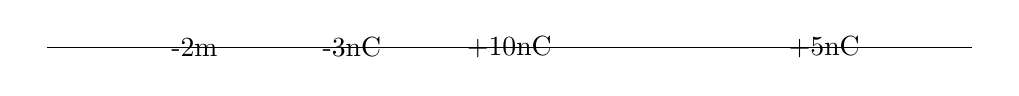
\begin{tikzpicture}
        [scale=2]
        \node (l1) at (-3,0) {};
        \node (l2) at (3,0) {};
        \node(a) at (-2, 0) {-2m};
        \node(b) at (-1,0) {-3nC};
        \node(c) at (0,0) {+10nC};
        \node(d) at (2,0) {+5nC};

        \draw[-] (l1) -- (l2);

    \end{tikzpicture}
    Finding $\overrightarrow{E}$: $\sum \overrightarrow{E} = \text{vector sum}$.
    \begin{align*}
        E_{-1} &= \frac{k(-3 \times 10^{-9})}{1} \\
        E_{0} &= \frac{k(10 \times 10^{-9})}{2^2} \\
        E_{+2} &= \frac{k(5 \times 10^{-9})}{4^2} \\
    \end{align*}
    Electric field points toward negative charges

    Negative at $-2m$ is different from the negative at $2m$. Points to the right at $-2$ and to the left at $2$. Sketch arrows on the line. Away from the negative charge, toward the positive charge. Positive in this Coulomb's Law means attraction. Positive means out from the center. Negative means in towards the center.

    $E = \frac{kQ}{r^2}$. $k = \frac{1}{4\pi \epsilon_0} \cdot \frac{Q}{r^2}$
    \begin{itemize}
        \item Epsilon naught is the permittivity of free space. Related to $c$.
        \item $4\pi$ comes from surface area of sphere.
        \item $\epsilon_0$ = 8.85 $\times 10^{-12}$
        \item $\sqrt{\epsilon_0 \mu_0} = c$
    \end{itemize}
    https://www.deepspace.ucsb.edu/wp-content/uploads/2010/08/033_Chapter-22-Flux-and-Gauss-Law-PML.pdf
\end{document}
